\documentclass{article} % For LaTeX2e
\usepackage{nips14submit_e,times}
\usepackage{graphicx}
\usepackage{hyperref}
\usepackage{url}
%\documentstyle[nips14submit_09,times,art10]{article} % For LaTeX 2.09


\nipsfinalcopy
\title{Employing an HMM and Decision Tree to Predict Student Behavior}

\author{
Maximo Q.~Menchaca\\
Department of Atmospheric Science\\
518 ATG\\
\texttt{menchaca@uw.edu} \\
\And
John G.~Lee\\
Department of Physics \\
180 NPL Building \\
\texttt{jgl6@uw.edu} \\
}

% The \author macro works with any number of authors. There are two commands
% used to separate the names and addresses of multiple authors: \And and \AND.
%
% Using \And between authors leaves it to \LaTeX{} to determine where to break
% the lines. Using \AND forces a linebreak at that point. So, if \LaTeX{}
% puts 3 of 4 authors names on the first line, and the last on the second
% line, try using \AND instead of \And before the third author name.

\newcommand{\fix}{\marginpar{FIX}}
\newcommand{\new}{\marginpar{NEW}}

%\nipsfinalcopy % Uncomment for camera-ready version

\begin{document}


\maketitle

\begin{abstract}
An online tutoring system tracks student interactions as they learn. The tracked interactions can be used to predict student performance. The method outlined in our project proposal [4] describes the beginnings of an HMM and decision tree to predict this performance. The decision tree and HMM will be used in conjunction to determine the learning rate of a student. While not yet used synergistically, both methods already yield promise in predicting student behavior.

\end{abstract}

\section{Data preprocessing}
The data comes in the format of records from the tutoring program, 19 variables. These variables include Problem Section, Unit, Name, time spent on the problem, hint queries, and number of times a student encounters a particular skill. Student IDs and problem information were converted from strings to integers, while dates were converted to epoch time. Because multiple skills could be present for an individual problem, Knowledge Component (KC) skills were converted to a matrix with component values set to one if the skill is present in the problem and zero otherwise. Similarly the associated Opportunity variable was converted to a matrix but with component values set to the opportunity number if the skill is present in the problem and zero otherwise.

\section{Decision Tree}
\subsection{Implementation}
The goal of a decision tree is to partition the data into classes that give low entropy organization of the dependent variable. Some variables lend themselves better to splitting then others. For example, one would expect the variable 'Opportunity' to be a good variable to split on - the more times a student encounters a given variable, the better they should do. Another possibility is 'Step Duration' - the longer a student spends on a given step, the more trouble they may be having and the less likely it is they will do well. On the other hand, the variable 'Incorrects' would be an extremely poor variable to split on - if a student achieved ANY incorrects for a given step, obviously they must not have gotten their first attempt correct!

\subsection{Test, Results}
We implement a preliminary decision tree using the two variables 'Step Duration' and 'Opportunity'. The following two tables depict the two possible trees with this implementation. The parenthetical values is the count in each class - and Root = Opportunity/Root = Step Duration give the predicted y value.
\begin{table}[t]
\caption{Decision tree application to test data}
\begin{center}
\begin{tabular}{c|c|c|c|c|c|c|c}
\multicolumn{8}{c}{Root = Opportunity}\\
Duration & Empty & 1 $>$ 5 & 5 $>$ 15 & 15 $>$ 25 & 25 $>$ 50 & 50 $>$ 100 & 100 $>$ ...\\
& (202669) & (66137) & (113527) & (73460) & (109617) & (105889) & (138395)\\
\hline
empty (3268) & 0/1 (1912) & 0/0 (245) & 0/0(301) & 0/0 (139) & 0/0 (222) & 0/0 (265) & 0/0 (184)\\
1 $>$ 15 (471730) & 1/0 (118157) & 1/0  (28966) & 1/0 (61024) & 1/0 (41988) & 1/0 (64766) & 1/0 (65678) & 1/0 (91151)\\
15 $>$ 30 (148490) & 0/0 (36914) & 0/0  (13167) & 0/0 (21686) & 0/0 (13453) & 0/0 (20447) & 0/0 (19060) & 0/0 (23763)\\
30 $>$ 45 (65065) & 0/0 (17430) & 0/0  (6766) & 0/0 (9919) & 0/0 (5941) & 0/0 (8564) & 0/0 (7586) & 0/0 (8859)\\
45 $>$ 60 (35206) & 0/0 (9043) & 0/0 (4086) & 0/0 (5599) & 0/0 (3426) & 0/0 (4582) & 0/0 (4035) & 0/0 (4435)\\
60 $>$ ... (85935) & 0/0 (19213) & 0/0 (12907) & 0/0 (14998) & 0/0 (8513) & 0/0 (11036) & 0/0 (9265) & 0/0 (10003)\\
\end{tabular}
\end{center}
\end{table}

The raw entropy of the data is $H(Y)$= 0.78, and after applying our decision tree, we obtain similar values either way - $H(Y|\bf{Opp}|\bf{Duration}) \approx H(Y|\bf{Duration}|\bf{Opp})$ = 0.65. However, we can see that the predicted values are much different either way - there is just one positive prediction if we use a root of Step Duration - when the opportunity is empty! This indicates some lack of robustness in choosing bins for the opportunity, which can be confirmed by changing these bins (not shown). On the other hand, we see that a small step duration leads to positive prediction robustly across all opportunity classes.

Applying this binning to create predicted $y_{pred}$ = 'Correct First Attempt' leads to an RMSE of $||y - y_{pred}||_2$ = .284 for Root = Opportunity and = .45 for Root = Step Duration across the training set. We cannot apply the decision tree on its own to the test set, as the step duration is not given.

\section{Hidden Markov Model}
\subsection{Implementation}
A hidden Markov model (HMM) was implemented to track the learning curve of the individual students [1]-[2]. We assume our hidden state is whether the student is knowledgeable or not at the time i in order to predict the probability of getting the problem i+1 correct on the first attempt. The model requires the creation of a finite set of possible observations given the various preprocessed variables. 

\subsection{Test}
We have experimented with smoothing by applying the forward-backward algorithm to predict subsequent Correct First Attempt variables. Educated but rough assumptions were made about start, transition, and emission probabilities of the hidden and observed states. Observations at a given problem are split into three states based on (1) whether their first attempt on any problem was correct; (2) if not, whether they at least had more corrects than incorrects over their entire observation history, and (3) otherwise. The students are assumed to start in the unknowledgeable state with 99\% probability. The smoothed data then predicts a probability for observing the next Correct on First Attempt variable as a 1.

\subsection{Results}
The output probabilities are plagued by underflows, where the probability of being in a particular hidden model state after many steps is too small to be tracked. A simple fix is to try implementing using an arbitrary floating point python package like mpmath. Another possibility is trying to implement the forward/backward algorithm with log probabilities instead [2]. Currently, underflow errors are treated as non-predictive, a state that currently applies to approximately a third of students, but predictive states show a root-mean-square-error of .477. A few quick tests were performed stepping through different transition probabilites from the unknowledgeable state, see figure~\ref{fig:dunno}.

\begin{figure}[h]
\begin{center}
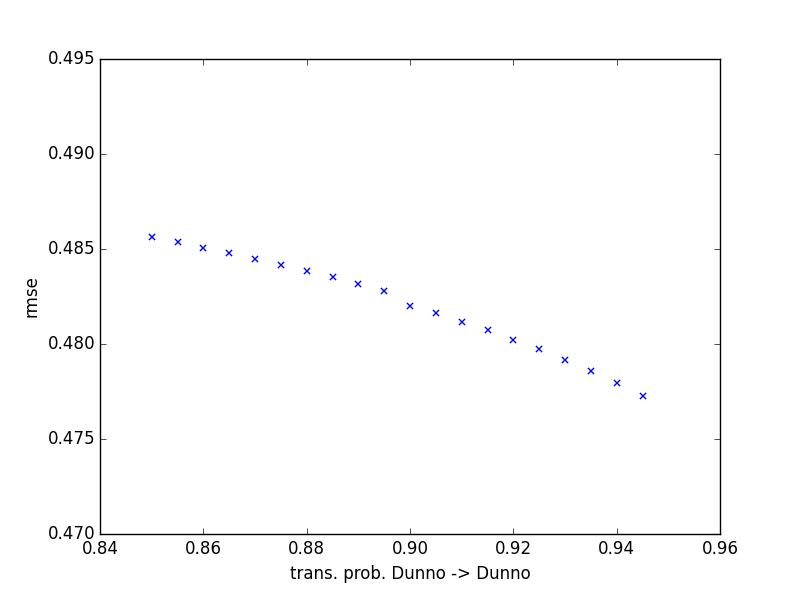
\includegraphics[width=0.8\textwidth]{dunno.png}
\label{fig:dunno}
\end{center}
\caption{Root-Mean-Square-Error with increasing probability of staying at unknowledgeable state from problem to problem.}
\end{figure}

\section{Future Work}

The decision tree on its own cannot be used on the test data, as very few variables are given (just the student, problem, opportunity, tested skill). We hope to implement the Baum-Welch algorithm to train our HMM transition and emission probabilities instead of the biased guesses used above. Additionally, we intend to implement these hidden Markov model algorithms not just on each student but for each skill a student encounters, to take advantage of data given in the test set. The decision tree will be implemented to further inform the transition probabilities used in the HMM. Variables deemed important in predicting a student's correct first attempt can be observed in test data and used to tune transition and emission probabilities - and finally, the time of transition to mastering a particular skill can be compared with the times in the test data to predict the student's correct attempts.

\subsubsection*{Acknowledgments}

Author MM acknowledges John G. Lee for his quality work thus far on the project described above. Author JL acknowledges Maximo Q. Menchaca for his quality work thus far on the project described above.

\subsubsection*{References}

\small{
[1] Frazzoli, E. (2010) Principles of Autonomy and Decision Making. 
\url{http://ocw.mit.edu/courses/aeronautics-and-astronautics/16-410-principles-of-autonomy-and-decision-making-fall-2010/lecture-notes/MIT16_410F10_lec21.pdf}\label{ref:hmmMIT}

[2] Domingos, P. (2015) \url{ http://courses.cs.washington.edu/courses/cse515/15wi/hmm.ppt}\label{ref:hmmUW}

[3] Hasselmo, M.E., Schnell, E. \& Barkai, E. (1995) Dynamics of learning
and recall at excitatory recurrent synapses and cholinergic modulation
in rat hippocampal region CA3. {\it Journal of Neuroscience}
{\bf 15}(7):5249-5262.
}

[4] Lee, J.G.\& Menchaca, M.Q. (2015) Student Performance Prediction Using Hidden Markov Models and Decision Tree. CSE 546 Autumn 2015 Project Proposal, 1 pp., Unpublished.

[5] Guestrin, C. (2014) \url{ https://courses.cs.washington.edu/courses/cse546/14au/slides/decision-trees-annotated.pdf}

\end{document}